\chapter{Computational Fluid Dynamics}
\chaptermark{CFD} %% this is the chapter heading that will show on subsequent pages

In this chapter I present the basics of CFD that will be necessary to understand our approach to modeling the thermosyphon numerically.
This consists of a derivation of the equations, and a discussion of their solution on a finite grid.

\section{Derivation of Governing Equations}

Closely following the original derivation of Stokes \shortcite{stokes}, I present a derivation of the main equations governing the flow of water at temperatures near 300K (an incompressible, heat-conducting, Newtonian fluid).

%% These three equations are given by
%% \begin{align*}
%% &\frac{\partial \rho}{\partial t} +
%% \frac{\partial}{\partial x_j}\left[ \rho u_j \right] = 0\\
%% &\frac{\partial}{\partial t}\left( \rho u_i \right) +
%% \frac{\partial}{\partial x_j}
%% \left[ \rho u_i u_j + p \delta_{ij} - \tau_{ji} \right] = 0, \quad i=1,2,3\\
%% &\frac{\partial}{\partial t}\left( \rho e_0 \right) +
%% \frac{\partial}{\partial x_j}
%% \left[ \rho u_j e_0 + u_j p + q_j - u_i \tau_{ij} \right] = 0\\
%% \end{align*}

%% Follow: \url{http://www.allstar.fiu.edu/aero/Flow2.htm} And \url{http://www.cfd-online.com/Wiki/Navier-Stokes_equations}

\subsection{Continuity Equation}

Considering a finite volume element with side lengths $\Delta x, \Delta y$ and $\Delta z$.
%% need be careful that this is a right handed coordinate system
The amount of mass that enters any given face on this volume is a function of the fluid density $\rho$, the velocity tangent to this face, and the area of the face.
For the a side with edges specified by both $\Delta x$ and $\Delta y$, let the velocity tangent to this face be $u$ and this mass flow in this side is equal to
$$ \rho u \Delta x \Delta y .$$
Assuming the $u$ is positive in this direction, the mass flux out of the opposite side needs to reflect possible changes in velocity $u$ and density $\rho$ through the volume and can be written
$$ -(\rho + \Delta \rho) (u+\Delta u) \Delta x \Delta y.$$
Similarly for the other two directions tangent to our volume, we assign velocities $v$ and $w$ with incoming mass
\begin{align*} &\rho v \Delta x \Delta z\\
&\rho w \Delta y \Delta z\end{align*}
and outgoing mass
\begin{align*} &-(\rho + \Delta \rho )( v+ \Delta v) \Delta x \Delta z\\
&-(\rho+\Delta \rho) (w+\Delta w) \Delta y \Delta z.\end{align*}
The rate of mass accumulation in the volume,
$$ \Delta \rho (\Delta x \Delta y \Delta z) / \Delta t, $$
must be equal to the sum of the mass entering and leaving the volume (given by the six equations above).
Equating these, with a little cancellation and dividing by $(\Delta x \Delta y \Delta z)$ we are left with
\begin{equation} \frac{\Delta \rho}{\Delta t} + \frac{\Delta (\rho u)}{\Delta x} + \frac{\Delta (\rho v)}{\Delta y} + \frac{\Delta (\rho w)}{\Delta z} = 0. \end{equation}
As $\Delta t \to 0$, this can be written in terms of the partial derivatives
\begin{equation} \frac{\partial \rho}{\partial t} + \frac{\partial (\rho u)}{\partial x} + \frac{\partial (\rho v)}{\partial y} + \frac{\partial (\rho w)}{\partial z} = 0. \label{eq:NScont} \end{equation}

For an incompressible fluid, we have that $\partial \rho / \partial \{ t,x,y,z\} = 0$ such the continuity equation becomes
\begin{equation} \frac{\partial u}{\partial x} + \frac{\partial v}{\partial y} + \frac{\partial w}{\partial z} = 0. \label{eq:NScontIco} \end{equation}

\subsection{Momentum Equation}

We now consider the second conservation law: the conservation of momentum.
This states that the rate of change of momentum must equal the net momentum flux into the control volume in addition to any external forces (e.g. gravity) on the control volume.
Again consider a small but finite volume element with side lengths $\Delta x, \Delta y$ and $\Delta z$.
Since the conservation of momentum applies in $x,y$ and $z$ directions, without loss of generality I consider only the $x$ direction.

The rate of change of momentum with respect to time in our volume element is
\begin{equation*} \frac{\partial }{\partial t} \left ( \rho u \right) \Delta x \Delta y \Delta z .\end{equation*}

The momentum flux into the volume in the $x$ direction is the mass flux times $x$-velocity, since momentum is mass$\times$velocity.
Recall the mass flux is given by $\rho u \times A$ for $A$ the area orthogonal to $x$, in this case $\Delta y \Delta z$.
Therefore the momentum flux is
\begin{equation*} u \times \rho u (\Delta y \Delta z) .\end{equation*}
Similarly, with the additional consideration of the change within the volume, the momentum flux leaving through the opposite side is
\begin{equation*} - \left ( u\rho u + \frac{\partial}{\partial x} \left( u\rho u\right ) \Delta x \right ) \Delta y \Delta z .\end{equation*}

The $y$ and $z$ direction momemtum flux (of $x$ direction momentum) is found in the same way and we have the fluxes in those directions as
\begin{align*} u \times \rho v (\Delta x \Delta z) & ~~~\& ~~~ - \left ( u\rho v + \frac{\partial}{\partial y} \left( u\rho v\right ) \Delta y \right ) \Delta x \Delta z \\
u \times \rho w (\Delta x \Delta y) & ~~~\& ~~~ - \left ( u\rho w + \frac{\partial}{\partial z} \left( u\rho w\right ) \Delta z \right ) \Delta x \Delta y . \end{align*}

Equating the change in internal momentum with the sum of the fluxes, and the sum of the external forces in the $x$ direction $\mathbf{F}_1$, we have the most basic form of the momentum equation:

\begin{align*} \frac{\partial }{\partial t} \left ( \rho u \right) \Delta x \Delta y \Delta z &= \frac{\partial }{\partial t} \left ( \rho u \right) \Delta x \Delta y \Delta z  - \left ( u\rho u + \frac{\partial}{\partial x} \left( u\rho u\right ) \Delta x \right ) \Delta y \Delta z +  u \rho v (\Delta x \Delta z) \\
& - \left ( u\rho v + \frac{\partial}{\partial y} \left( u\rho v\right ) \Delta y \right ) \Delta x \Delta z + u \rho w (\Delta x \Delta y)\\
& - \left ( u\rho w + \frac{\partial}{\partial z} \left( u\rho w\right ) \Delta z \right ) \Delta x \Delta y + \sum \mathbf{F}_1.\end{align*}

Cancelling the first terms from each flux we are left
\begin{align*} \frac{\partial }{\partial t} \left ( \rho u \right) \Delta x \Delta y \Delta z &=  -  \frac{\partial}{\partial x} \left( u\rho u\right ) \Delta x  \Delta y \Delta z - \frac{\partial}{\partial y} \left( u\rho v\right ) \Delta y \Delta x \Delta z\\
& - \frac{\partial}{\partial z} \left( u\rho w\right ) \Delta z \Delta x \Delta y + \sum \mathbf{F}_1.\end{align*}

Pulling out the $\Delta x \Delta y \Delta z$ and moving just the forces to the right we have

\begin{align*} \Delta x \Delta y \Delta z \left (\frac{\partial }{\partial t} \left ( \rho u \right)  +  \frac{\partial}{\partial x} \left( u\rho u\right )  + \frac{\partial}{\partial y} \left( u\rho v\right ) +\frac{\partial}{\partial z} \left( u\rho w\right ) \right ) &= \sum \mathbf{F}_1.\end{align*}

Applying the product rule to the partial derivatives with respect to $x,y$ and $z$ we find the continuity equation which we know to be zero, and are left
\begin{align*} \Delta x \Delta y \Delta z \left ( \rho \frac{\partial u }{\partial t} + \rho u \frac{\partial u }{\partial x} + \rho v \frac{\partial u}{\partial y} + \rho w \frac{\partial u}{\partial z} \right ) &= \sum \mathbf{F}_1 .\end{align*}

The sum of the forces in the $x$ direction includes the force of gravity that acts on the mass of the entire volume ($g_1 \times \rho \Delta x\Delta y \Delta z$) and the surface stress.
We assume that gravity acts only in the $z$ direction where the term $g_3 \times \rho \Delta x \Delta y \Delta z$ shows up in the sum of the forces and is otherwise zero.
The $x$-direction force of the stresses acting on the volume is the product of the stress and the area on which it acts, and in cartesian coordinates this is either direct or shear stress.
The $x$-normal stress, which we denote $s_{xx}$ has forces on both sides tangent to $x$ given by
\begin{equation*} s_{xx} \Delta y \Delta z ~~~\& ~~~ \left ( s_{xx} + \frac{\partial s_{xx} }{\partial x} \Delta x \right ) \Delta y \Delta z \end{equation*}
for which the sum is
\begin{equation*} \frac{\partial s_{xx} }{\partial x} \Delta x \Delta y \Delta z .\end{equation*}
The forces of the shear stress on the faces planar to $x$ are similarly
\begin{equation*} \frac{\partial s_{yx} }{\partial x} \Delta x \Delta y \Delta z ~~~\&~~~\frac{\partial s_{zx} }{\partial x} \Delta x \Delta y \Delta z .\end{equation*} 

Since the pressure $p$ does not apply shear stress, $p$ is only a part of $s_{xx}$ and not $s_{yx},s_{zx}$.
In each direction we denote the viscous stress as $\tau _{ij}$ for $i$ and $j$ the directions $x,y,$ and $z$.
Thus for general fluids the sum of the forces in the $x$ direction is
\begin{equation*} \left ( \frac{\partial p }{\partial x} + \frac{\partial \tau _{xx}}{\partial x} + \frac{\partial \tau _{yx}}{\partial y} + \frac{\partial \tau _{zx}}{\partial z} \right ) \Delta x \Delta y \Delta z . \end{equation*}

Since the thermosyphon is filled with water, not blood, we can happily assume that the fluid is Newtonian, and the rapture has been avoided.
This means that we can relate the viscous stress to the local rate of deformation linearly, by the viscocity $\mu$:
\begin{align*} \tau _{xx} &= 2 \mu \frac{\partial u}{\partial x} \\
\tau _{yx} &= \mu \left ( \frac{\partial v}{\partial x} + \frac{\partial u}{\partial y} \right )\\
\tau _{zx} &= \mu \left ( \frac{\partial w}{\partial x} + \frac{\partial u}{\partial z} \right )\end{align*}

Putting this together for our Newtonian fluid we have by the equality of mixed partials and the continuity equation we have the sum of all the forces given by
\begin{align*} & \left (-\frac{\partial p}{\partial x} + 2 \mu \frac{\partial u}{\partial x^2} + \mu \frac{\partial}{\partial y} \frac{\partial v}{\partial x} + \mu \frac{\partial }{\partial y} \frac{\partial u}{\partial y} + \mu \frac{\partial }{\partial z} \frac{\partial u}{\partial z} + \mu \frac{\partial }{\partial z} \frac{\partial w}{\partial x}\right ) \Delta x \Delta y \Delta z\\
& = \left ( -\frac{\partial p}{\partial x} + \mu \frac{\partial u}{\partial x^2} + \mu\frac{\partial u}{\partial y^2} + \mu \frac{\partial u}{\partial z^2}  + \mu \frac{\partial u}{\partial x^2} + \mu \frac{\partial}{\partial x} \frac{\partial v}{\partial y} + \mu \frac{\partial }{\partial x} \frac{\partial w}{\partial z} \right ) \Delta x \Delta y \Delta z\\
& = \left (-\frac{\partial p}{\partial x} + \mu \frac{\partial u}{\partial x^2} + \mu\frac{\partial u}{\partial y^2} + \mu \frac{\partial u}{\partial z^2}  + \mu \frac{\partial }{\partial x}\left ( \frac{\partial u}{\partial x} + \frac{\partial v}{\partial y} + \frac{\partial w}{\partial z} \right ) \right ) \Delta x \Delta y \Delta z\\
& = \left ( -\frac{\partial p}{\partial x} + \mu \frac{\partial u}{\partial x^2} + \mu\frac{\partial u}{\partial y^2} + \mu \frac{\partial u}{\partial z^2}\right ) \Delta x \Delta y \Delta z\end{align*}

Thus the momemtum equation for $x$ is
\begin{align}  \rho \left ( \frac{\partial u }{\partial t} + u \frac{\partial u }{\partial x} + v \frac{\partial u}{\partial y} + w \frac{\partial u}{\partial z} \right ) &= -\frac{\partial p}{\partial x} + \mu \frac{\partial u}{\partial x^2} + \mu\frac{\partial u}{\partial y^2} + \mu \frac{\partial u}{\partial z^2}\end{align}

In tensor notation this is often written for all three equations (recall, the above is only for $x$):

\begin{equation} \rho \frac{\partial u_i}{\partial t} + \frac{\partial}{\partial x_j} \left( u_j u_i \right) = -\frac{\partial p}{\partial x_i}  + \mu \frac{\partial u_i}{\partial x_j^2}  + \rho g_i . \end{equation}

Working our way towards OpenFOAM's implementation of this equation, write the filtered equation for averaged quantities of pressure $\bar{p}$, density $\bar{\rho}$ and velocity $\bar{u}$, and assume that the density is constant except for when multiplied by gravitational effects, writing $\bar{\rho} = \overline{\rho} / \rho _0$:

\begin{equation} \rho _0 \left ( \frac{\partial \bar{u}_i}{\partial t} + \frac{\partial}{\partial x_j} \left( \bar{u}_j \bar{u}_i \right) \right )
= -\frac{\partial \bar{p}} {\partial{x_i}} +  \mu \frac{\partial \bar{u}_i}{\partial x_j^2} + \bar{\rho} g_i. \end{equation}

Since we will be relying on the use of a turbulence model, we reintroduce the stress tensor $\tau _{ij}$ and split $\tau_{ij}$ into the mean stress tensor $\tau _{ij}$ and the turbulent stress tensor $\tau ^* _{ij}$.
In tensor notation the mean stress tensor can be written
\begin{equation*} \tau _{ij} = \mu \left ( \left ( \frac{\partial \bar{u} _i}{\partial x_j} + \frac{\partial \bar{u} _j }{\partial x_i} \right) - \frac{2}{3} \frac{\partial \bar{u}_k} {\partial x_k} \delta _{ij} \right ) \end{equation*}
for $\delta _{ij} = 0$ if and only if $i=j$.
Assume constant viscocity $\mu = \mu _0$, divide by $\rho _0$ and incorporate the latter for the stress tensor and we now have the momentum equation as
\begin{equation*} \frac{\partial \bar{u}_i}{\partial t} + \frac{\partial}{\partial x_j} \left( \bar{u}_j \bar{u}_i \right) 
= -\frac{\partial } {\partial{x_i}} \frac{\bar{p}}{\rho_0} + \frac{\partial }{\partial x_j} \left ( \nu _0 \left ( \left ( \frac{\partial \bar{u}_i} {\partial x_j} + \frac{\partial \bar{u} _j}{\partial x_i} \right ) - \frac{2}{3}\left ( \frac{\partial \bar{u} _k}{\partial x_k }\right ) \delta _{ij}\right ) - \tau ^* _{ij} \right ) + \bar{\rho} g_i \end{equation}
where $\nu _0 = \mu _0 /\rho _0$.
We can then decompose the turbulent stress tensor $\tau ^* _{ij}$ further using $R_{ij}$ to denote the Reynolds stress tensor
\begin{equation*} \tau ^* _{ij} = R_{ij} = R^D _{ij} + \frac{2}{3} k \delta _{ij} \end{equation*}
for $R_{ij}^D$ the deviatoric part and $k = R_{ii}/2$ the turbulent kinetic energy.
For LES this becomes the sub-grid kinetic energy.
Note that OpenFOAM outputs the resolved kinematic pressure
\begin{equation*} \tilde{p} = \frac{\bar{p} }{\rho _0} + \frac{2}{3}k \end{equation}
and uses the Boussinesq approximation for the last term
\begin{equation*} g_i\frac{\bar{\rho}}{\rho _0} = g_i \left ( 1 + \frac{\bar{\rho} - \rho _0}{\rho _0} \right ) = g_i \rho _k  = g_i (1 - \beta \left (\overline{T} - T _0\right ) .\end{equation}

\subsection{Energy Equation}

Again following the derivation of Anderson, we derive the energy equation into the form used in OpenFOAM \shortcite{anderson2009governing}.
Since our problem deals with an incompressible fluid, we are only concerned with the temperature parts of the energy equation and begin with this consideration to greatly simplify the derivation.

The temperature (energy) equation is thus
\begin{equation} \frac{\partial }{\partial t} \left ( \rho e\right ) + \frac{\partial}{\partial x_j} \left ( \rho e u_j \right ) 
= 
%% -p \frac{\partial u_k}{\partial x_k} + %% zero due to conservation law
%% \tau _{ij} \frac{\partial u_i}{\partial x_j} %% zero for incompressible fluid
- \frac{\partial q_k}{\partial x_k}
\end{equation}
for $e$ the internal energy and $q$ the conductive heat flux.
Averaging this equation and separting the heat flux into the average and turbulent parts $q = \overline{q} + q^*$ we have
\begin{equation} \frac{\partial }{\partial t} \left ( \rho \overline{e}\right ) + \frac{\partial}{\partial x_j} \left ( \rho \overline{e} \overline{u}_j \right ) 
= 
- \frac{\partial q_k^*}{\partial x_k}
- \frac{\partial \overline{q}_k}{\partial x_k}
\end{equation}

\section{Discretization and Solving Algorithms}

A spatial and temporal discretization of the governing equations is necessary for their solution numerically.
In general, there are three approaches to the solution of PDE's numerically: finite differences, finite element, and finite volume.
OpenFOAM has the capacity for each scheme, and for our problem the finite volume method is most appropriate.
%% The principle disadvantage 

After discretization, solving is accomplished by a combined SIMPLE/PISO algorithm.
The PISO (Pressure-Implicit with Splitting of Operators) algorithm derives from the work of \shortcite{issa1986solution}, and is complementary to the SIMPLE (Semi-Implicit Method for Pressure-Linked Equations) \shortcite{patankar1972calculation} iterative method.

Simple algorithm:
\url{http://www.cfd-online.com/Wiki/SIMPLE_algorithm}

The proper inclusion of turbulent effects with calculated Raleigh number are important, and are modeled using LES (Large Eddy Simulation).

\section{Solving with OpenFOAM}

Using the aforementioned numerical schemes, I perform a computational fluid dynamic simulation of the entire thermosyphon using the open-source software OpenFOAM.
First, we begin by creating 2 and 3-dimensional meshes of the thermosyphon natively in OpenFOAM's blockMesh utility.
To reduce computational bandwidth, it was important to first create the mesh and then renumber using the renumberMesh utility.
The 2D mesh contains 36000 points, and is imposed with fixed flux boundary conditions on the top and bottom of the loop.
This fixed flux boundary condition is implemented through the externalWallHeatFluxTemperature library, with some difficulty.
The 3D mesh contains over 1M points, and we have chosen to explore the 2D model for now.
Mesh refinement near walls is important to capture the physics happening at the wall on finer scales, and this is achieved adaptively through the refineMesh utility.



Links for OpenFOAM code documentation:

\url{http://www.openfoam.org/docs/user/compiling-applications.php}

\url{http://www.openfoam.org/docs/cpp/}

Here is a picture of the thermosyphon colored by temperature.
\begin{figure}[tpb!]
  \centering
  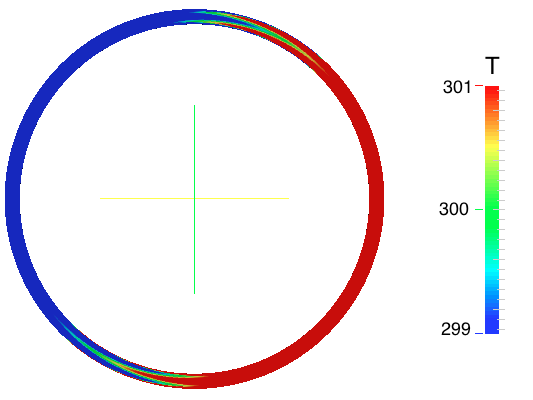
\includegraphics[width=0.49\textwidth]{figures/loop-screenshot.png}
  \caption{
  A screenshot of the loop.
  }
  \label{fig:CFDloopSS}
\end{figure}

And here is the 2D mesh:
\begin{figure}[tpb!]
  \centering
  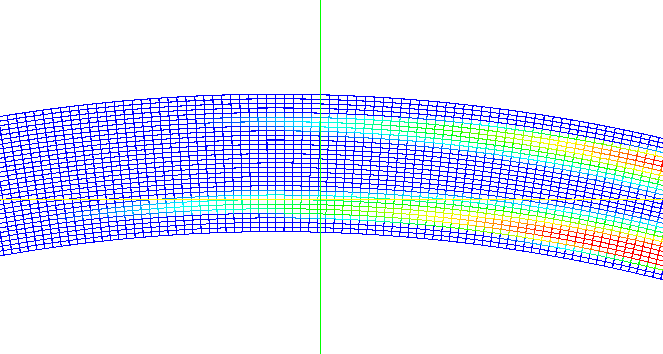
\includegraphics[width=0.49\textwidth]{figures/mesh.png}
  \caption{
  A snapshot of the mesh used for CFD simulations.
  }
  \label{fig:CFDmesh1}
\end{figure}

The solver used is buoyantBoussinesqPimpleFoam, which I'll now explain. 

The Boussinesq approximation makes the assumption that density changes due to temperature differences are sufficiently small so that they can be neglected without affecting the flow, except when multiplied by gravity.
The non-dimensionalized density difference $\Delta \rho / \rho$ depends on the value of heat flux into the loop, but remains small even for large values of flux. (derive an equation for this ratio in terms of flux $q''$).

Available boundary conditions that were found to be stable in OpenFOAM's solver were both constant gradient and fixed value conditions.
To most accurately model our our experiment, we choose a fixed value BC.
This is reasonable given the thermal diffusivity of the walls of the convection loop and their thickness.
[Derive condition]



